\chapter{Cubos e blocos retangulares}\label{ch:g5:solids}

Saindo da página plana: os \omterm{def:g5:solids:def}{sólidos} são as formas do mundo real ---
dados, caixas de cereal, latas, bolas. Este capítulo aprende a
nomeá-los, a contar as \omterm{def:g5:solids:def}{faces} e as \omterm{def:g5:solids:def}{arestas} deles, a desdobrá-los em
planificações e a medir o \omterm{def:g5:solids:volume}{volume} contando cubinhos. (As fórmulas de
\omterm{def:g5:solids:volume}{volume} vêm no \cref{ch:g6:measure}.)

\section{A família dos sólidos}

\begin{definition}[Os sólidos e o vocabulário deles]\label{def:g5:solids:def}
Um \emph{sólido}\index{sólido} ocupa espaço. Os lados planos são as
\emph{faces}\index{face}; as faces se encontram nas
\emph{arestas}\index{aresta}; as arestas se encontram nos
\emph{vértices}\index{vértice}. Os retratos de família:
\begin{itemize}
  \item o \emph{cubo}\index{cubo}: $6$ faces quadradas, $12$ arestas,
        $8$ vértices;
  \item o \emph{bloco retangular}\index{bloco retangular} (prisma de
        base retangular): $6$ faces retangulares, $12$ arestas, $8$
        vértices;
  \item o \emph{cilindro}\index{cilindro}: duas faces em forma de disco e uma face
        enrolada (uma lata);
  \item a \emph{pirâmide}\index{pirâmide}: uma base poligonal e triângulos que se
        encontram num ápice;
  \item a \emph{bola} (esfera): uma superfície perfeitamente redonda,
        sem face e sem aresta.
\end{itemize}
\end{definition}

\begin{omfigure}
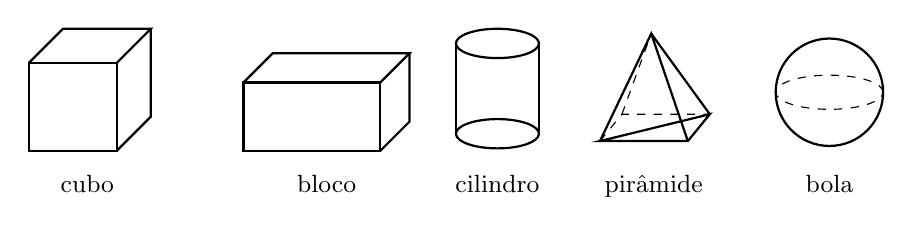
\begin{tikzpicture}[scale=0.62]
  % cubo
  \draw[thick] (0,0) rectangle (1.8,1.8);
  \draw[thick] (0,1.8) -- (0.7,2.5) -- (2.5,2.5) -- (1.8,1.8);
  \draw[thick] (2.5,2.5) -- (2.5,0.7) -- (1.8,0);
  \node[below, font=\small] at (1.2,-0.3) {cubo};
  % bloco
  \begin{scope}[xshift=4.4cm]
  \draw[thick] (0,0) rectangle (2.8,1.4);
  \draw[thick] (0,1.4) -- (0.6,2.0) -- (3.4,2.0) -- (2.8,1.4);
  \draw[thick] (3.4,2.0) -- (3.4,0.6) -- (2.8,0);
  \node[below, font=\small] at (1.7,-0.3) {bloco};
  \end{scope}
  % cilindro
  \begin{scope}[xshift=9.6cm]
  \draw[thick] (0,0.35) ellipse (0.85 and 0.3);
  \draw[thick] (-0.85,0.35) -- (-0.85,2.2);
  \draw[thick] (0.85,0.35) -- (0.85,2.2);
  \draw[thick] (0,2.2) ellipse (0.85 and 0.3);
  \node[below, font=\small] at (0,-0.3) {cilindro};
  \end{scope}
  % pirâmide
  \begin{scope}[xshift=12.6cm]
  \draw[thick] (-0.9,0.2) -- (0.9,0.2) -- (1.35,0.75) -- cycle;
  \draw[thick] (-0.9,0.2) -- (0.15,2.4) -- (0.9,0.2);
  \draw[thick] (1.35,0.75) -- (0.15,2.4);
  \draw[dashed] (-0.9,0.2) -- (-0.45,0.75) -- (1.35,0.75);
  \draw[dashed] (-0.45,0.75) -- (0.15,2.4);
  \node[below, font=\small] at (0.2,-0.3) {pirâmide};
  \end{scope}
  % bola
  \begin{scope}[xshift=16.4cm]
  \draw[thick] (0,1.2) circle (1.1);
  \draw[dashed] (0,1.2) ellipse (1.1 and 0.35);
  \node[below, font=\small] at (0,-0.3) {bola};
  \end{scope}
\end{tikzpicture}

{\small A galeria dos \omterm{def:g5:solids:def}{sólidos}. As linhas tracejadas mostram as
\omterm{def:g5:solids:def}{arestas} escondidas --- o fundo do \omterm{def:g5:solids:def}{sólido}, visto através dele.}
\end{omfigure}

\begin{example}[Contar no cubo]\label{ex:g5:solids:count}
Confira num dado: $6$ \omterm{def:g5:solids:def}{faces} (os números de $1$ a $6$), $8$ \omterm{def:g5:solids:def}{vértices}
(os cantos), $12$ \omterm{def:g5:solids:def}{arestas} (passe o dedo por elas: $4$ em cima, $4$
embaixo, $4$ verticais). E $6 + 8 = 12 + 2$ --- o mesmo padrão
curioso vale para o bloco e para a \omterm{def:g5:solids:def}{pirâmide} (o
\cref{ex:g8:solids:count} volta a ele).
\end{example}

\section{Planificações}

\begin{definition}[Planificação]\label{def:g5:solids:net}
Uma \emph{planificação}\index{planificação} de um \omterm{def:g5:solids:def}{sólido} é um desenho
plano de todas as \omterm{def:g5:solids:def}{faces} dele, unidas pelas \omterm{def:g5:solids:def}{arestas}, que se dobra e
forma o \omterm{def:g5:solids:def}{sólido} --- o \omterm{def:g5:solids:def}{sólido} desembrulhado, como uma caixa de papelão
achatada para a reciclagem.
\end{definition}

\begin{omfigure}
\begin{tikzpicture}[scale=0.5]
  \draw[gray!40, thin] (0,0) grid (4,3);
  \draw[thick, omDef] (0,1) rectangle (1,2);
  \draw[thick, omDef] (1,1) rectangle (2,2);
  \draw[thick, omDef] (2,1) rectangle (3,2);
  \draw[thick, omDef] (3,1) rectangle (4,2);
  \draw[thick, omDef] (1,2) rectangle (2,3);
  \draw[thick, omDef] (1,0) rectangle (2,1);
  \node[below, font=\small] at (2,-0.5) {uma planificação do cubo};
  \begin{scope}[xshift=7.5cm]
  \draw[gray!40, thin] (0,0) grid (4,3);
  \draw[thick, omThm] (0,1) rectangle (1,2);
  \draw[thick, omThm] (1,1) rectangle (2,2);
  \draw[thick, omThm] (2,1) rectangle (3,2);
  \draw[thick, omThm] (3,1) rectangle (4,2);
  \draw[thick, omThm] (0,2) rectangle (1,3);
  \draw[thick, omThm] (0,0) rectangle (1,1);
  \node[below, font=\small] at (2,-0.5) {outra planificação válida};
  \end{scope}
  \begin{scope}[xshift=15cm]
  \draw[gray!40, thin] (0,0) grid (4,3);
  \draw[thick, omExo] (0,1) rectangle (1,2);
  \draw[thick, omExo] (1,1) rectangle (2,2);
  \draw[thick, omExo] (2,1) rectangle (3,2);
  \draw[thick, omExo] (3,1) rectangle (4,2);
  \draw[thick, omExo] (0,2) rectangle (1,3);
  \draw[thick, omExo] (1,2) rectangle (2,3);
  \node[below, font=\small] at (2,-0.5) {não é planificação! (por quê?)};
  \end{scope}
\end{tikzpicture}

{\small Três arranjos de seis quadrados. Os dois primeiros se dobram
num \omterm{def:g5:solids:def}{cubo}; o terceiro não --- ao dobrar, dois quadrados caem sobre a
mesma \omterm{def:g5:solids:def}{face} e o \omterm{def:g5:solids:def}{cubo} fica aberto. Recorte e experimente!}
\end{omfigure}

\begin{example}[Ler uma planificação]\label{ex:g5:solids:read}
Num dado, as \omterm{def:g5:solids:def}{faces} opostas somam $7$. Na \omterm{def:g5:solids:net}{planificação}, as \omterm{def:g5:solids:def}{faces}
opostas são as separadas por exatamente um quadrado numa fileira (ou
dobrando um canto) --- não as vizinhas! Marcar os pares na
\omterm{def:g5:solids:net}{planificação} antes de dobrar é um ótimo exercício de enxergar o
espaço no plano.
\end{example}

\section{Volume: contar cubinhos}

\begin{definition}[Volume por contagem]\label{def:g5:solids:volume}
O \emph{volume}\index{volume} de um \omterm{def:g5:solids:def}{sólido} montado com cubinhos
unitários é o número de cubinhos que ele contém. A unidade pode ser o
centímetro cúbico (cm$^3$) ou o metro cúbico (m$^3$).
\end{definition}

\begin{example}[Contar um bloco camada por camada]\label{ex:g5:solids:layers}
Um bloco com $4$ cubinhos de comprimento, $3$ de largura e $2$ de
altura: a camada de baixo leva $4 \times 3 = 12$ cubinhos, e há $2$
camadas:
\[
12 \times 2 = 24 \text{ cubinhos} .
\]
Contar por camadas sempre funciona --- e demonstra discretamente a
fórmula $V = L \times w \times h$ do \cref{ch:g6:measure}.
\end{example}

\begin{omfigure}
\begin{tikzpicture}[scale=0.52]
  \foreach \y in {0,1} {
    \foreach \x in {0,...,3} {
      \foreach \z in {0,1,2} {
        \begin{scope}[shift={({\x+0.4*\z},{\y+0.28*\z})}]
          \draw[fill=omDef!12] (0,0) rectangle (1,1);
          \draw[fill=omDef!22] (0,1) -- (0.4,1.28) -- (1.4,1.28)
            -- (1,1) -- cycle;
          \draw[fill=omDef!30] (1,0) -- (1.4,0.28) -- (1.4,1.28)
            -- (1,1) -- cycle;
        \end{scope}
      }
    }
  }
  \node[below, font=\small] at (2.6,-0.4)
    {$4 \times 3$ cubinhos por camada, $2$ camadas: $24$ cubinhos};
\end{tikzpicture}

{\small Um bloco $4 \times 3 \times 2$ de cubinhos unitários, contado
camada por camada.}
\end{omfigure}

\begin{example}[Os mesmos cubinhos, formas diferentes]\label{ex:g5:solids:rearrange}
Oito cubinhos unitários montam um \omterm{def:g5:solids:def}{cubo} $2 \times 2 \times 2$, um
bastão $8 \times 1 \times 1$ ou uma laje $4 \times 2 \times 1$: três
\omterm{def:g5:solids:def}{sólidos} diferentes, um só \omterm{def:g5:solids:volume}{volume} ($8$ cubinhos). O \omterm{def:g5:solids:volume}{volume} conta o
material, não a forma.
\end{example}

\section{Exercícios}

\begin{exercise}[$\star$]\label{exo:g5:solids:1}
Dê o nome de um objeto real com o formato de: um \omterm{def:g5:solids:def}{cubo}; um \omterm{def:g5:solids:def}{bloco
retangular}; um \omterm{def:g5:solids:def}{cilindro}; uma bola; uma \omterm{def:g5:solids:def}{pirâmide}.
\end{exercise}

\begin{exercise}[$\star$]\label{exo:g5:solids:2}
Quantas \omterm{def:g5:solids:def}{faces}, \omterm{def:g5:solids:def}{arestas} e \omterm{def:g5:solids:def}{vértices} tem um \omterm{def:g5:solids:def}{bloco retangular}? Confira o
padrão \omterm{def:g5:solids:def}{faces} $+$ \omterm{def:g5:solids:def}{vértices} $=$ \omterm{def:g5:solids:def}{arestas} $+ 2$.
\end{exercise}

\begin{exercise}[$\star$]\label{exo:g5:solids:3}
Que \omterm{def:g5:solids:def}{faces} de um \omterm{def:g5:solids:def}{bloco retangular} são idênticas? (Agrupe as seis \omterm{def:g5:solids:def}{faces}
em pares.) O que há de especial nas \omterm{def:g5:solids:def}{faces} do \omterm{def:g5:solids:def}{cubo}?
\end{exercise}

\begin{exercise}[$\star$]\label{exo:g5:solids:4}
Trace uma \omterm{def:g5:solids:net}{planificação} de um \omterm{def:g5:solids:def}{cubo} de lado $2$ cm (use o modelo em
forma de cruz do capítulo), recorte-a e dobre-a.
\end{exercise}

\begin{exercise}[$\star$]\label{exo:g5:solids:5}
Na \omterm{def:g5:solids:net}{planificação} em cruz de um dado, coloque os números de $1$ a $6$
de modo que as \omterm{def:g5:solids:def}{faces} opostas somem $7$. (Use o
\cref{ex:g5:solids:read} para achar antes os pares opostos.)
\end{exercise}

\begin{exercise}[$\star$]\label{exo:g5:solids:6}
Conte os cubinhos unitários: um bloco de $5$ de comprimento, $2$ de
largura e $3$ de altura; um \omterm{def:g5:solids:def}{cubo} de lado $3$; uma pilha em forma de L
feita de uma laje $3 \times 2 \times 1$ com uma laje
$1 \times 2 \times 1$ em cima.
\end{exercise}

\begin{exercise}[$\star$]\label{exo:g5:solids:7}
Um bloco leva exatamente $12$ cubinhos unitários numa camada. Dê dois
formatos possíveis de camada ($L \times w$) e, para cada um, o \omterm{def:g5:solids:volume}{volume}
do bloco se ele tiver $3$ camadas dessas.
\end{exercise}

\begin{exercise}[$\star$]\label{exo:g5:solids:8}
Com $27$ cubinhos unitários, que \omterm{def:g5:solids:def}{cubo} você consegue montar? E com
$64$? (Pense na contagem por camadas ao contrário.)
\end{exercise}

\begin{exercise}[$\star\star$]\label{exo:g5:solids:9}
Torrões de açúcar de lado $1$ cm vêm numa caixa de $10$ cm de
comprimento, $5$ cm de largura e $4$ cm de altura (medidas internas).
Quantos torrões cabem? Se uma família usa $6$ torrões por dia, para
quantos dias dura uma caixa (arredonde com bom senso)?
\end{exercise}

\begin{exercise}[$\star\star$]\label{exo:g5:solids:10}
Um \omterm{def:g5:solids:def}{cubo} $3 \times 3 \times 3$ é pintado de vermelho por fora e depois
cortado em $27$ cubinhos unitários. Quantos cubinhos têm tinta em
exatamente $3$ \omterm{def:g5:solids:def}{faces}? Em $2$? Em $1$? Em nenhuma? (Confira: as quatro
contagens têm de somar $27$.)
\end{exercise}
